% Practice Test 18 — Vermont Edition
% Questions: 30 (26 MC + 4 SA)
% Generated by scripts/generate_practice_tests.py

\begin{practiceQuestion}{1-3-q12}{mc}
\begin{questionText}
A proportional table has $k = \frac{3}{4}$. Which pair could be in the table?
\end{questionText}
\choiceA{$(8, 10)$}
\choiceB{$(8, 6)$}
\choiceC{$(12, 8)$}
\choiceD{$(4, 2)$}
\correctAnswer{B}
\explanation{If $k = \frac{3}{4}$, then $y = \frac{3}{4}x$. For $x = 8$: $y = \frac{3}{4} \times 8 = 6$. So $(8, 6)$ works.}
\end{practiceQuestion}

\begin{practiceQuestion}{1-5-q04}{mc}
\begin{questionText}
Two proportional lines are graphed. Line A is steeper than Line B. What does this tell you?
\end{questionText}
\choiceA{Line A has a smaller unit rate}
\choiceB{Line A has a greater unit rate}
\choiceC{Line B covers more distance}
\choiceD{Both lines have the same rate}
\correctAnswer{B}
\explanation{A steeper line means a higher slope, which equals a greater unit rate (constant of proportionality).}
\end{practiceQuestion}

\begin{practiceQuestion}{1-6-q12}{mc}
\begin{questionText}
Store A sells $3$ notebooks for $\$7.50$. Store B sells $5$ notebooks for $\$11.25$. Which store offers the better deal?
\end{questionText}
\choiceA{Store A at $\$2.50$ each}
\choiceB{Store B at $\$2.25$ each}
\choiceC{Store A at $\$2.25$ each}
\choiceD{They cost the same}
\correctAnswer{B}
\explanation{Store A: $7.50 \div 3 = \$2.50$ each. Store B: $11.25 \div 5 = \$2.25$ each. Store B is cheaper.}
\end{practiceQuestion}

\begin{practiceQuestion}{2-1-q12}{mc}
\begin{questionText}
$63$ is $90\%$ of what number?
\end{questionText}
\choiceA{$56.7$}
\choiceB{$67$}
\choiceC{$70$}
\choiceD{$72$}
\correctAnswer{C}
\explanation{Divide: $63 \div 0.90 = 70$.}
\end{practiceQuestion}

\begin{practiceQuestion}{2-5-q11}{mc}
\begin{questionText}
Estimate a $15\%$ tip on a $\$78$ bill using the $10\%$ method.
\end{questionText}
\choiceA{About $\$7.80$}
\choiceB{About $\$10.40$}
\choiceC{About $\$11.70$}
\choiceD{About $\$15.60$}
\correctAnswer{C}
\explanation{$10\%$ of $\$78 = \$7.80$. Half of that ($5\%$) $= \$3.90$. Add: $7.80 + 3.90 = \$11.70$.}
\end{practiceQuestion}

\begin{practiceQuestion}{2-7-q02}{mc}
\begin{questionText}
A student measured a table as $4.5$ feet long. The actual length is $5$ feet. What is the percent error?
\end{questionText}
\choiceA{$0.5\%$}
\choiceB{$5\%$}
\choiceC{$10\%$}
\choiceD{$11.1\%$}
\correctAnswer{C}
\explanation{$\frac{|4.5 - 5|}{5} \times 100 = \frac{0.5}{5} \times 100 = 10\%$.}
\end{practiceQuestion}

\begin{practiceQuestion}{3-1-q13}{mc}
\begin{questionText}
For which value of $n$ is $|n| = 10$?
\end{questionText}
\choiceA{Only $n = 10$}
\choiceB{Only $n = -10$}
\choiceC{$n = 10$ or $n = -10$}
\choiceD{$n = 0$}
\correctAnswer{C}
\explanation{Both $|10| = 10$ and $|-10| = 10$. Two numbers have the same absolute value: the number and its opposite.}
\end{practiceQuestion}

\begin{practiceQuestion}{3-2-q03}{mc}
\begin{questionText}
What is $15 + (-15)$?
\end{questionText}
\choiceA{$30$}
\choiceB{$-30$}
\choiceC{$15$}
\choiceD{$0$}
\correctAnswer{D}
\explanation{A number plus its opposite (additive inverse) always equals $0$.}
\end{practiceQuestion}

\begin{practiceQuestion}{4-1-q14}{mc}
\begin{questionText}
What is the value of $x^2 + 3x$ when $x = -2$?
\end{questionText}
\choiceA{$10$}
\choiceB{$-2$}
\choiceC{$-10$}
\choiceD{$2$}
\correctAnswer{B}
\explanation{Substitute: $(-2)^2 + 3(-2) = 4 + (-6) = -2$.}
\end{practiceQuestion}

\begin{practiceQuestion}{4-2-q12}{mc}
\begin{questionText}
Simplify $-6y + 4y - y$.
\end{questionText}
\choiceA{$-3y$}
\choiceB{$-y$}
\choiceC{$3y$}
\choiceD{$-11y$}
\correctAnswer{A}
\explanation{$-6y + 4y = -2y$. Then $-2y - y = -3y$.}
\end{practiceQuestion}

\begin{practiceQuestion}{5-2-q11}{mc}
\begin{questionText}
Solve $9 + 3x = 30$.
\end{questionText}
\choiceA{$x = 13$}
\choiceB{$x = 3$}
\choiceC{$x = 7$}
\choiceD{$x = 10$}
\correctAnswer{C}
\explanation{Subtract $9$: $3x = 21$. Divide by $3$: $x = 7$. Check: $9 + 3(7) = 9 + 21 = 30$ \checkmark.}
\end{practiceQuestion}

\begin{practiceQuestion}{5-3-q25}{sa}
\begin{questionText}
Solve $9(x - 3) = 45$.
\end{questionText}
\correctAnswer{$x = 8$}
\explanation{Divide by $9$: $x - 3 = 5$. Add $3$: $x = 8$. Check: $9(8 - 3) = 9(5) = 45$ \checkmark.}
\end{practiceQuestion}

\begin{practiceQuestion}{5-4-q06}{mc}
\begin{questionText}
Solve $-0.4y + 2 = 6$.
\end{questionText}
\choiceA{$y = 10$}
\choiceB{$y = -10$}
\choiceC{$y = 20$}
\choiceD{$y = -20$}
\correctAnswer{B}
\explanation{Subtract $2$: $-0.4y = 4$. Divide by $-0.4$: $y = -10$. Check: $-0.4(-10) + 2 = 4 + 2 = 6$ \checkmark.}
\end{practiceQuestion}

\begin{practiceQuestion}{5-5-q20}{sa}
\begin{questionText}
Solve $-5n + 10 \leq -15$.
\end{questionText}
\correctAnswer{$n \geq 5$}
\explanation{Subtract $10$: $-5n \leq -25$. Divide by $-5$ and flip: $n \geq 5$.}
\end{practiceQuestion}

\begin{practiceQuestion}{5-6-q14}{mc}
\begin{questionText}
Solve $-3x + 12 \geq 0$ and describe the graph.
\end{questionText}
\choiceA{Closed circle at $4$, shade right}
\choiceB{Open circle at $4$, shade left}
\choiceC{Closed circle at $4$, shade left}
\choiceD{Closed circle at $-4$, shade right}
\correctAnswer{C}
\explanation{Subtract $12$: $-3x \geq -12$. Divide by $-3$ and flip: $x \leq 4$. Closed circle at $4$, shade left.}
\end{practiceQuestion}

\begin{practiceQuestion}{6-2-q17}{mc}
\begin{questionText}
A map uses $1$ cm $= 60$ km. You redraw it at $1$ cm $= 20$ km. A triangle on the original has an area of $4$ cm$^2$. What is its area on the new map?
\end{questionText}
\choiceA{$12$ cm$^2$}
\choiceB{$16$ cm$^2$}
\choiceC{$36$ cm$^2$}
\choiceD{$48$ cm$^2$}
\correctAnswer{C}
\explanation{Scale ratio: $\frac{60}{20} = 3$. Area scales by $3^2 = 9$. New area: $4 \times 9 = 36$ cm$^2$.}
\end{practiceQuestion}

\begin{practiceQuestion}{6-3-q27}{gmc}
\begin{questionText}
The diagram shows a triangle with the given measurements. How many different triangles can be drawn with these exact conditions?

\begin{center}
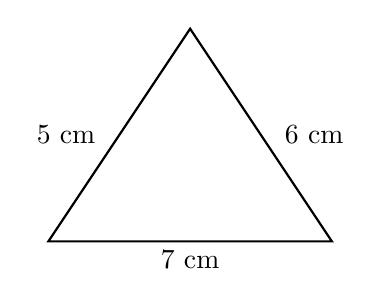
\begin{tikzpicture}[scale=0.9]
  \draw[thick] (0,0) -- (4,0) -- (2,3) -- cycle;
  \node[below] at (2,0) {$7$ cm};
  \node[left] at (0.8,1.5) {$5$ cm};
  \node[right] at (3.2,1.5) {$6$ cm};
\end{tikzpicture}
\end{center}
\end{questionText}
\choiceA{None}
\choiceB{Exactly one}
\choiceC{Exactly two}
\choiceD{Infinitely many}
\correctAnswer{B}
\explanation{Three side lengths that satisfy the triangle inequality (SSS) produce exactly one unique triangle. Check: $5 + 6 = 11 > 7$, $5 + 7 = 12 > 6$, $6 + 7 = 13 > 5$. All pass.}
\end{practiceQuestion}

\begin{practiceQuestion}{6-4-q09}{mc}
\begin{questionText}
A triangle has angles $90°$, $45°$, and $45°$. Which statement is true?
\end{questionText}
\choiceA{Exactly one such triangle exists}
\choiceB{Many triangles with these angles exist, in different sizes}
\choiceC{No such triangle exists because two angles are equal}
\choiceD{No such triangle exists because the angles don't sum to $180°$}
\correctAnswer{B}
\explanation{$90 + 45 + 45 = 180°$ \checkmark. But AAA alone allows different sizes. Many $45$-$45$-$90$ triangles exist.}
\end{practiceQuestion}

\begin{practiceQuestion}{6-5-q17}{mc}
\begin{questionText}
A triangular prism is sliced with a vertical cut perpendicular to the triangular bases. What shape is the cross-section?
\end{questionText}
\choiceA{Triangle}
\choiceB{Rectangle}
\choiceC{Circle}
\choiceD{Trapezoid}
\correctAnswer{B}
\explanation{A vertical cut perpendicular to the triangular bases of a triangular prism produces a rectangle (the cut goes through the lateral faces).}
\end{practiceQuestion}

\begin{practiceQuestion}{7-3-q11}{mc}
\begin{questionText}
A circular rug has a diameter of $8$ feet. What is the area of the rug? Use $\pi \approx 3.14$.
\end{questionText}
\choiceA{$25.12$ ft$^2$}
\choiceB{$50.24$ ft$^2$}
\choiceC{$200.96$ ft$^2$}
\choiceD{$64$ ft$^2$}
\correctAnswer{B}
\explanation{$r = 8 \div 2 = 4$ ft. $A = \pi r^2 = 3.14 \times 16 = 50.24$ ft$^2$.}
\end{practiceQuestion}

\begin{practiceQuestion}{7-4-q16}{mc}
\begin{questionText}
A figure is made of a right triangle with legs $6$ cm and $8$ cm, and a rectangle $8$ cm by $3$ cm. What is the total area?
\end{questionText}
\choiceA{$24$ cm$^2$}
\choiceB{$48$ cm$^2$}
\choiceC{$36$ cm$^2$}
\choiceD{$72$ cm$^2$}
\correctAnswer{B}
\explanation{Triangle: $\frac{1}{2} \times 6 \times 8 = 24$ cm$^2$. Rectangle: $8 \times 3 = 24$ cm$^2$. Total: $24 + 24 = 48$ cm$^2$.}
\end{practiceQuestion}

\begin{practiceQuestion}{7-5-q29}{gsa}
\begin{questionText}
The net shown below folds into a rectangular prism. Find the total surface area.

\begin{center}
\begin{tikzpicture}[scale=0.35]
  \draw[thick,funBlue,fill=funBlue!10] (0,0) rectangle (10,4);
  \draw[thick,funBlue,fill=funBlue!10] (10,0) rectangle (14,4);
  \draw[thick,funBlue,fill=funBlue!10] (14,0) rectangle (24,4);
  \draw[thick,funBlue,fill=funBlue!10] (24,0) rectangle (28,4);
  \draw[thick,funBlue,fill=funBlue!10] (0,4) rectangle (10,8);
  \draw[thick,funBlue,fill=funBlue!10] (0,-4) rectangle (10,0);
  % Dimensions
  \draw[thick,funRed,<->] (0,-5) -- (10,-5);
  \node[below,funRed] at (5,-5) {$10$ cm};
  \draw[thick,funRed,<->] (10,-5) -- (14,-5);
  \node[below,funRed] at (12,-5) {$4$};
  \draw[thick,funRed,<->] (-1,0) -- (-1,4);
  \node[left,funRed] at (-1,2) {$4$ cm};
\end{tikzpicture}
\end{center}
\end{questionText}
\correctAnswer{$192$ cm$^2$}
\explanation{The prism is $10 \times 4 \times 4$. $SA = 2(10 \times 4) + 2(10 \times 4) + 2(4 \times 4) = 80 + 80 + 32 = 192$ cm$^2$.}
\end{practiceQuestion}

\begin{practiceQuestion}{7-6-q18}{mc}
\begin{questionText}
A trapezoidal prism has a trapezoidal base with parallel sides $4$ cm and $6$ cm, height $3$ cm, and the prism length is $10$ cm. What is its volume?
\end{questionText}
\choiceA{$60$ cm$^3$}
\choiceB{$120$ cm$^3$}
\choiceC{$150$ cm$^3$}
\choiceD{$180$ cm$^3$}
\correctAnswer{C}
\explanation{$B = \frac{1}{2}(4 + 6) \times 3 = 15$ cm$^2$. $V = 15 \times 10 = 150$ cm$^3$.}
\end{practiceQuestion}

\begin{practiceQuestion}{8-1-q12}{mc}
\begin{questionText}
Which of the following increases the reliability of conclusions drawn from a sample?
\end{questionText}
\choiceA{Using a smaller sample}
\choiceB{Using a larger random sample}
\choiceC{Surveying only people who agree with you}
\choiceD{Using a non-random sample}
\correctAnswer{B}
\explanation{Larger random samples better represent the population and give more reliable results.}
\end{practiceQuestion}

\begin{practiceQuestion}{8-3-q18}{mc}
\begin{questionText}
School A: median score $88$, MAD $4$. School B: median score $82$, MAD $4$. The difference in medians expressed in MADs is:
\end{questionText}
\choiceA{$1$ MAD}
\choiceB{$1.5$ MADs}
\choiceC{$2$ MADs}
\choiceD{$4$ MADs}
\correctAnswer{B}
\explanation{Difference in medians: $88 - 82 = 6$. In MADs: $\frac{6}{4} = 1.5$ MADs.}
\end{practiceQuestion}

\begin{practiceQuestion}{8-4-q22}{sa}
\begin{questionText}
Group X: mean $45$, MAD $6$. Group Y: mean $57$, MAD $6$. Express the difference in means as a multiple of MAD.
\end{questionText}
\correctAnswer{$2$ MADs}
\explanation{Difference: $57 - 45 = 12$. In MADs: $\frac{12}{6} = 2$.}
\end{practiceQuestion}

\begin{practiceQuestion}{9-1-q18}{mc}
\begin{questionText}
Jasmine says the probability of picking a vowel from the letters of the word MATH is $\frac{2}{4}$. Is she correct?
\end{questionText}
\choiceA{Yes, because there are $2$ vowels in MATH}
\choiceB{No, there is only $1$ vowel in MATH, so the probability is $\frac{1}{4}$}
\choiceC{No, the probability is $\frac{3}{4}$}
\choiceD{Yes, because half of all letters are vowels}
\correctAnswer{B}
\explanation{The letters in MATH are M, A, T, H. Only A is a vowel. $P = \frac{1}{4}$.}
\end{practiceQuestion}

\begin{practiceQuestion}{9-4-q03}{mc}
\begin{questionText}
A bag contains $4$ red marbles and $1$ blue marble. Which type of probability model does this represent?
\end{questionText}
\choiceA{Uniform}
\choiceB{Non-uniform}
\choiceC{Both uniform and non-uniform}
\choiceD{Neither}
\correctAnswer{B}
\explanation{The probability of drawing red ($\frac{4}{5}$) is different from drawing blue ($\frac{1}{5}$), so this is a non-uniform model.}
\end{practiceQuestion}

\begin{practiceQuestion}{9-6-q04}{mc}
\begin{questionText}
Two dice are rolled. What is the probability of getting a sum of $2$?
\end{questionText}
\choiceA{$\frac{1}{6}$}
\choiceB{$\frac{1}{12}$}
\choiceC{$\frac{1}{36}$}
\choiceD{$\frac{2}{36}$}
\correctAnswer{C}
\explanation{The only way to get a sum of $2$ is $(1,1)$. $P = \frac{1}{36}$.}
\end{practiceQuestion}

\begin{practiceQuestion}{9-7-q15}{mc}
\begin{questionText}
You simulate flipping a coin $3$ times and counting how many times all $3$ are heads. In $40$ simulations, all $3$ heads occurs $6$ times. What is the experimental probability?
\end{questionText}
\choiceA{$\frac{6}{40} = 0.15$}
\choiceB{$\frac{1}{8} = 0.125$}
\choiceC{$\frac{3}{40} = 0.075$}
\choiceD{$\frac{6}{120} = 0.05$}
\correctAnswer{A}
\explanation{$P = \frac{6}{40} = 0.15$. The theoretical probability is $\frac{1}{8} = 0.125$, close to the simulation result.}
\end{practiceQuestion}
